\subsection{Model Details}
\label{sec:details}

%% Under the context of advertisement traffic estimation, it can be interpreted as:
%% \begin{itemize}
%% \item Similar advertisers are likely to have similar traffic ratios
%%   between the same pair of keywords, i.e. $\beta_{uj}/\beta_{ui}
%%   \approx \beta_{vj}/\beta_{vi}$ where $u$ and $v$ are ``similar''
%%   adgroups.
%% \item Similar keywords are likely to have similar entry value ratios
%%   between the same pair of advertisers, i.e. $\beta_{vi}/\beta_{ui}
%%   \approx \beta_{vj}/\beta_{uj}$ where $i$ and $j$ are ``similar''
%%   criteria.
%% \end{itemize}

There are two sets of parameters in {\sppan} model. One set is used to
capture the similarity between different advertisement. The other set
is used to weigh the importance of different ratios between keywords
when calculating estimates. Please refer to the example in
Section~\ref{sec:intuition}. Therefore, use data structure {\it
  Similarity Graph} to represent the first set of parameters, and {\it
  Pairwise Amplifier Graph} to represent the second set.

{\bf Similarity Graph} is the graph which describes the similarity
between different advertisers. To be more specific, it is a complete
undirected graph $G_{\mbox{sim}}=<V,E>$, where $V$ is the set of all
the advertisers. For each edge in $E$, there is a value which
represents how similar the corresponding two advertisers are with each
other. Let $\theta_{uv}$ denote the similarity between advertiser
$u$ and $v$.

%% \begin{comment}
%% % this graph does not provide much useful information, but a normal graph structure
%%  Figure~\ref{fig:sim-graph} shows an example fragment of the Similarity Graph.
%% \begin{figure}[!ht]
%%   \centering
%%   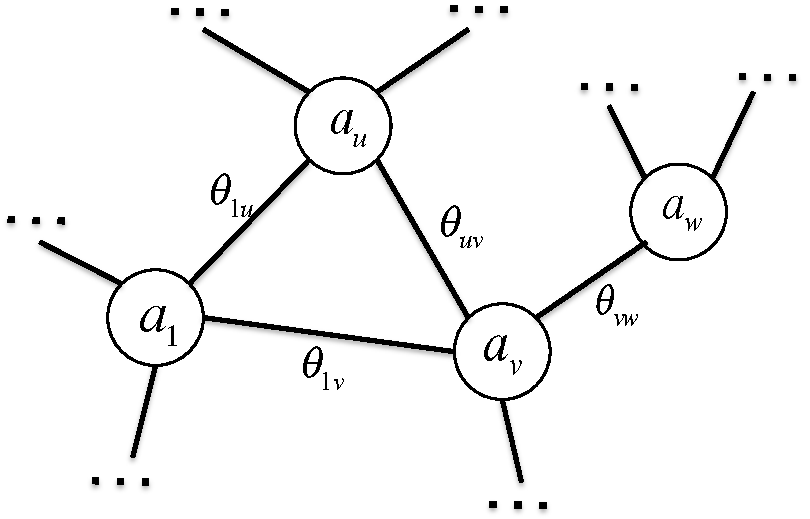
\includegraphics[width=0.35\textwidth]{figures/sim_graph.pdf}
%%   \caption{Similarity Graph}
%%   \label{fig:sim-graph}
%% \end{figure}
%% \end{comment}

{\bf Pairwise Amplifier Graph} contains all the ratio information
between different pairs of keywords. It is defined as a directed graph
$G_{\mbox{amp}}=<V,E>$, where $V$ contains all the keywords , and $E$
contains all pairs of keywords that have been targeted concurrently in
at least one advertisement, $E=\{(i,j)~|~ i\in [1,N_k],j \in
[1,N_k],\exists u\in [1,N_a]\mbox{ s.t. }\beta_{ui},\beta_{uj}\in
\Gamma\}$. For each edge $(i,j)\in E$, there are a corresponding
confidence value $conf_{ij}$ and an amplifier set
$amp_{ij}=\{(a_u,\gain{u}{ij})~|~u\in [1,N_a],\beta_{ui},\beta_{uj}\in
\Gamma\} \cup \{(a_0,c_{ij})\}$, where
$\gain{u}{ij}=\beta_{uj}/\beta_{ui}$, and $(a_0,c_{ij})$ are just the
bias terms which we will use later in the model.

\begin{comment}
 Figure~\ref{fig:amp-graph} shows an example fragment of the Pairwise
 Amplifier Graph.

\begin{figure}[!ht]
  \centering
  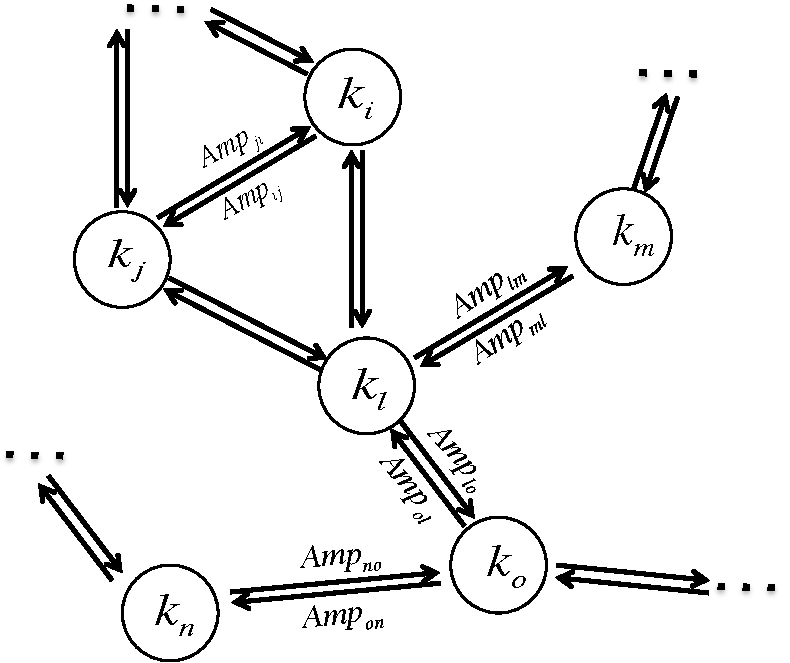
\includegraphics[width=0.35\textwidth]{figures/amp_graph.pdf}
  \caption{Pairwise Amplifier Graph}
  \label{fig:amp-graph}
\end{figure}
\end{comment}
